%%%%%%%%%%%%%%%%%%%%%%%%%%%%%%%%%
% Laatste aanpassing: 
% 5/1/14 [Jan]: oplossing oefening loften aangepast (suggestie Inge)
%
% 26/06/13 [Greetje]: Oefeningen van Leentje toegevoegd
% 18/2/12 [Jan]: Oef 7 aangepast
%
% 2/2/11 [Greetje]: nieuwe oefeningen toegevoegd. Formulering van sommige oefeningen aangepast.
%
% 14/09/10 [Greetje]: opgaven in 3 veranderlijken verwijderd. Herhalingsvragen weggelaten.
%
% 11/9/07 [Jan]: enkele fouten verbeterd
%          
% 14/9/05 [Jan]: vraag is 10 stoelen (i.p.v. 30)
%
% 8/09/01 door Greetje
%   correcties van Roos en Roby
%
% nieuwe aanpassing: 8/06/02 door Roos  %
%  nieuwe opgaven en volgorde veranderd       %
%%%%%%%%%%%%%%%%%%%%%%%%%%%%%%%%%

\section{Oefeningen}
\begin{oef}
De Indische regering kondigt een ambitieus plan aan om in
ieders voedselbehoefte te kunnen voorzien op basis van rijst en
sojascheuten. E\'{e}n kopje ongekookte rijst kost \euros{0,20} en bevat
15 gr eiwitten, 810 calorie\"{e}n en $\frac{1}{9}$ mg vitaminen
B2. E\'{e}n kopje sojascheuten kost \euros{0,40} en
levert 22,5 gr eiwitten, 270 calorie\"{e}n en $\frac{1}{3}$ mg
B2. Veronderstel dat de minimale dagelijkse
behoeften er als volgt uitzien: 90 gr eiwitten, 1620 calorie\"{e}n
en 1 mg vitamine B2.
Hoe ziet het goedkoopste
dieet dat voldoet aan de minimale behoeften eruit?
\begin{opl}
  De goedkoopste oplossing (figuur~\ref{fig:oplrijstsoja}) die aan alle beperkingen voldoet is drie kopjes rijst en twee kopjes sojascheuten, met een kostprijs van \euros{1,40}. 
  \begin{figure}[hbtp]
    \centering
    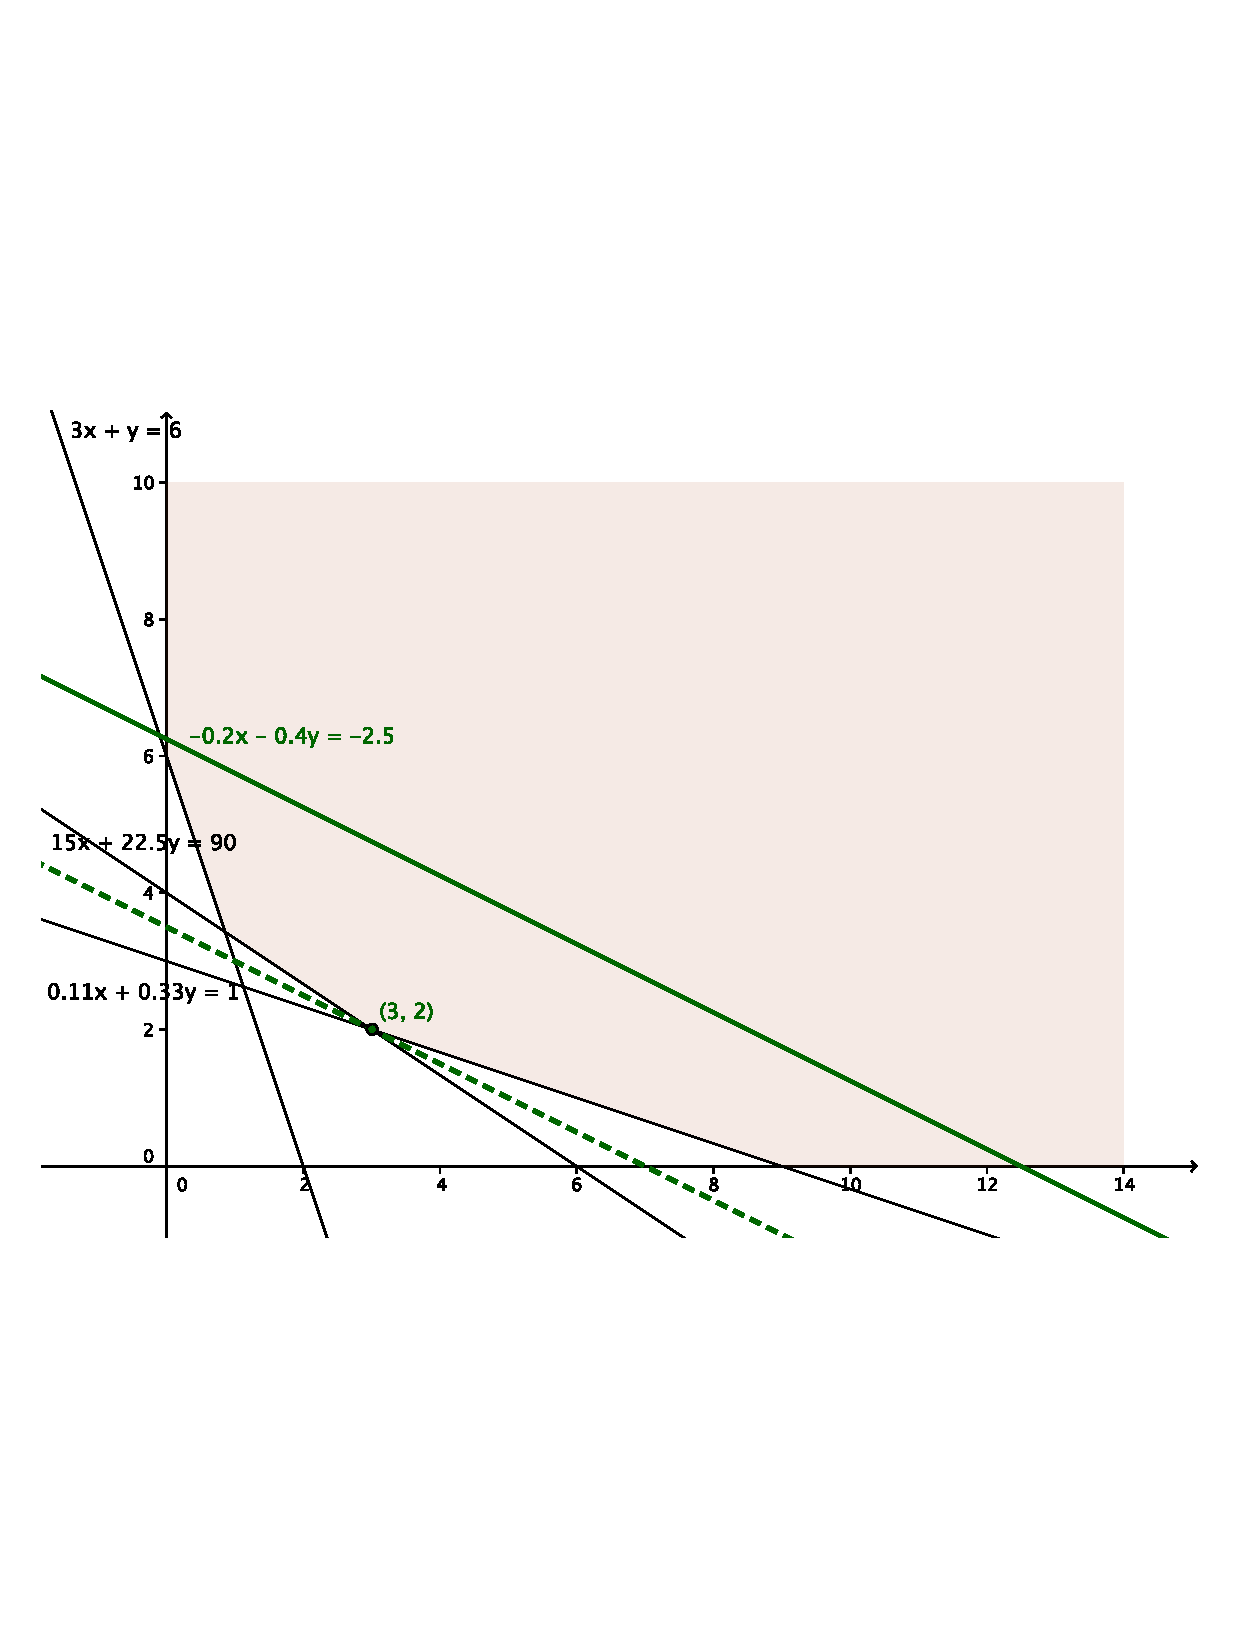
\includegraphics[width=0.8\textwidth]{oefeningen/FigurenLP/OefRijstSoja.pdf}
    \caption{Optimaal punt is drie kopjes rijst en twee kopjes soja}
    \label{fig:oplrijstsoja}
  \end{figure}
\end{opl}
\end{oef}
 
\begin{oef}
In een bedrijf worden nieuwe archiefkasten aangekocht. Er
is keuze tussen 2 types met verschillende afmetingen en
functies. Type A kost \euros{150} en is \SI{60}{\cm} diep, \SI{40}{\cm} breed en
\SI{1}{\m} hoog. Type B kast kost het dubbele van A maar is \SI{45}{\cm}
diep, \SI{80}{\centi\meter} breed en \SI{1,5}{\meter} hoog. Voor elke type A kast moeten
minstens 2 kasten van type B geplaatst worden. De totale
grondoppervlakte die in het bedrijf moet ingenomen worden door
archiefkasten is minstens \SI{3,84}{\square\meter}. Er is in totaal \euros{7500}
voorzien voor de aankoop. Hoeveel kasten van elk type moeten
er aangekocht worden om de kostprijs zo laag mogelijk te houden? 
\begin{opl}
Vier kasten van type A en acht kasten van type  B leveren de goedkoopste prijs van \euros{3000} en voldoen aan alle voorwaarden (figuur~\ref{fig:kastenAB}).
\begin{figure}[hbtp]
  \centering
  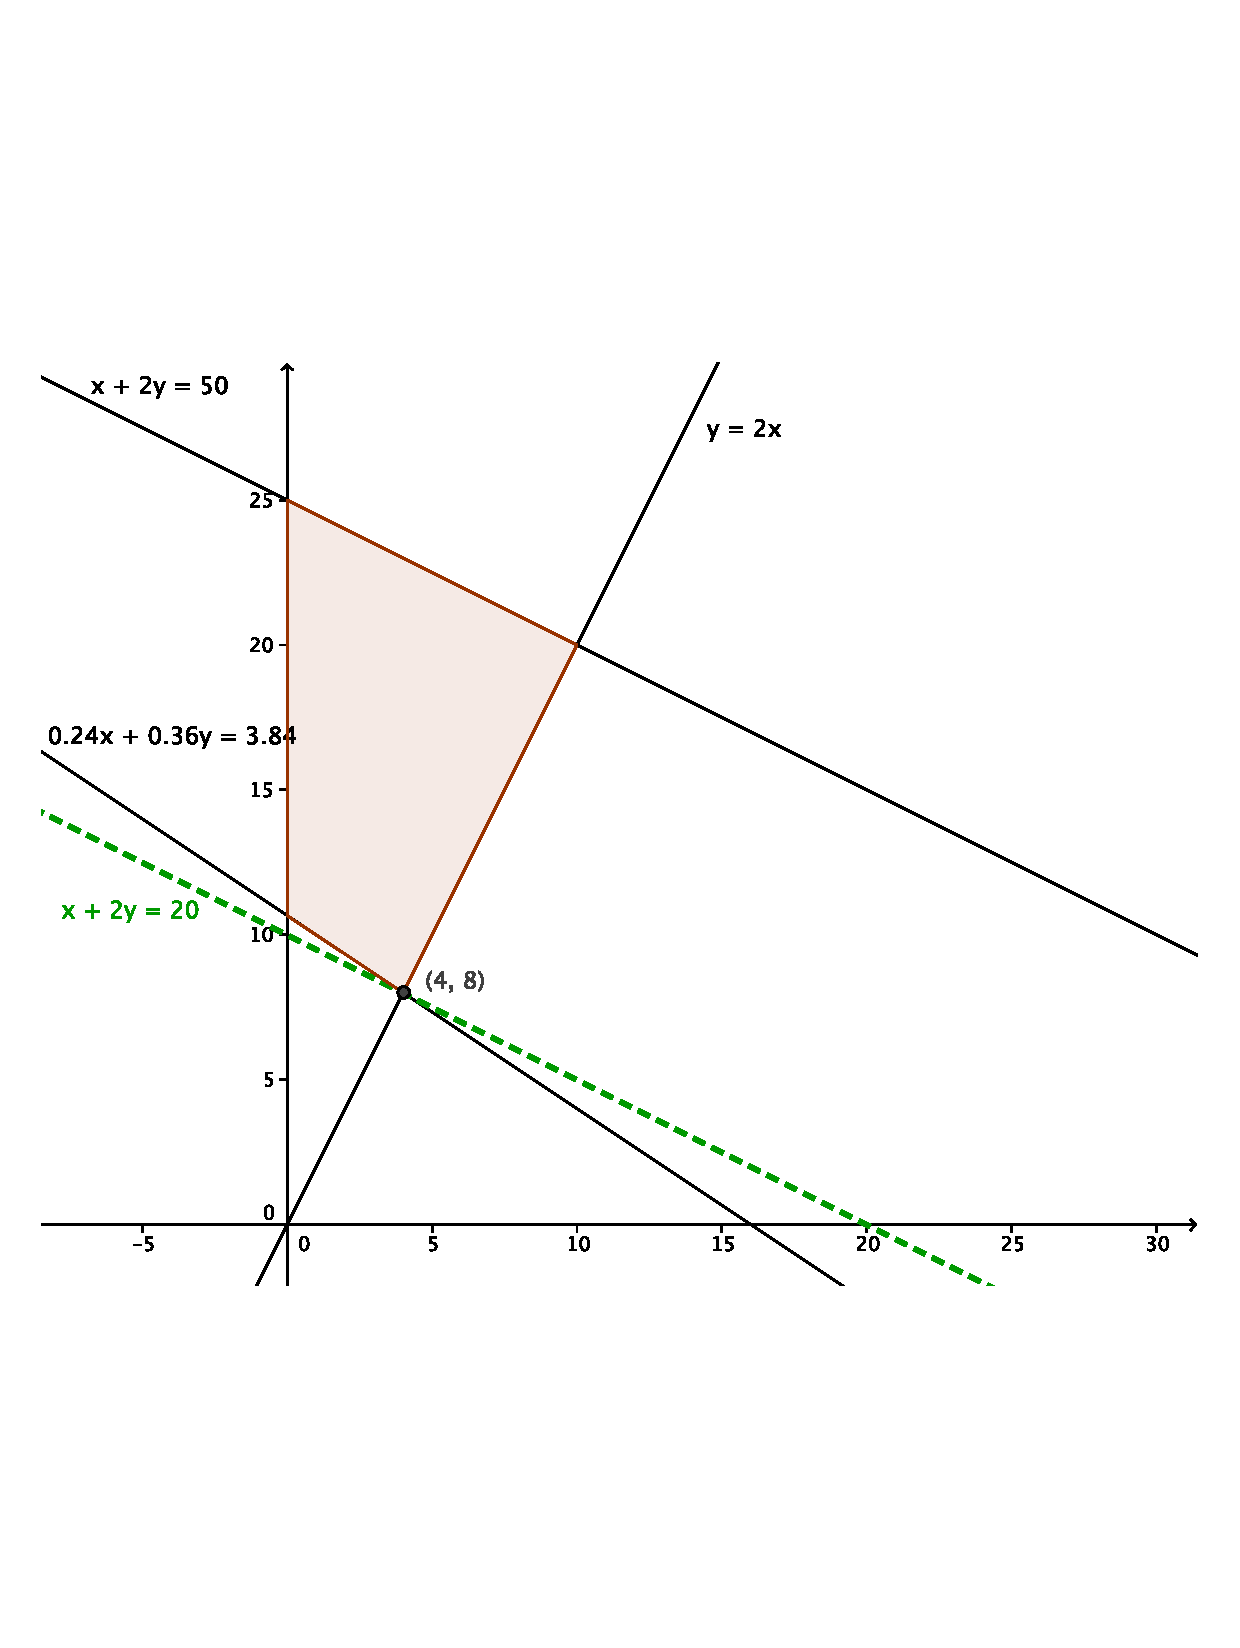
\includegraphics[width=0.8\textwidth]{oefeningen/FigurenLP/OefkastenAB.pdf}
  \caption{Optimaal punt is vier kasten A en acht kasten B}
  \label{fig:kastenAB}
\end{figure}
\end{opl}
\end{oef}
     
     
   
\begin{oef}
Het departement G\&T wordt verkozen tot `Departement van het
jaar'. Als beloning mogen alle personeelsleden en studenten -- in
totaal 2000 mensen -- gratis voor  \'e\'en week op reis naar
Kreta. `Cobol Airlines' zorgt voor het transport. 
\begin{figure}[h]
\centering
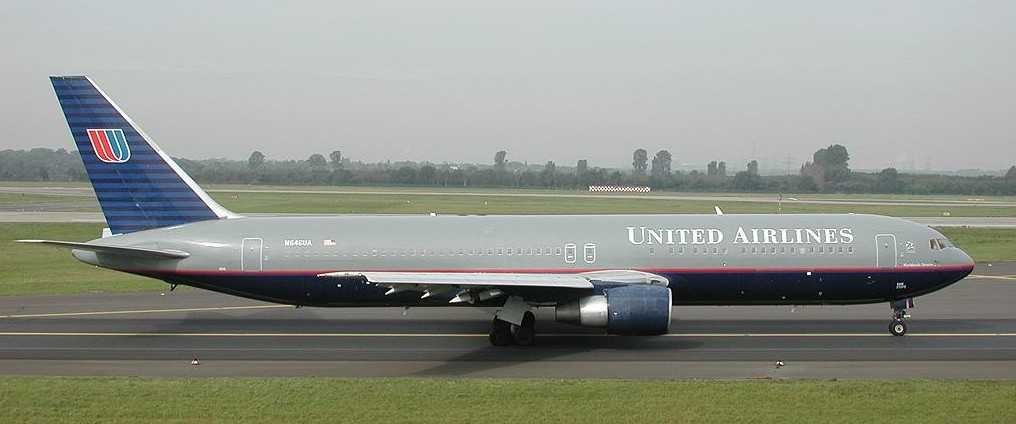
\includegraphics[width=0.8\textwidth]{oefeningen/FigurenLP/Boeing-767.jpg}
\caption{Boeing 767-300}
\end{figure}
Deze luchtvaartmaatschappij beschikt over een vloot van Fokkers en
Boeings 767. De Fokker heeft een capaciteit van 80 passagiers,
heeft 3 stewards aan boord en kost per vlucht \euros{20\,000}. De
Boeing 767 kan 240 personen meenemen, vraagt 4 Stewards en kost
\euros{100\,000} per vlucht.`Cobol Airlines' beschikt over 50
stewards. Er moeten minstens evenveel Fokkers als Boeings
ingezet worden voor het vervoer van deze 2000 mensen.
Wat is de samenstelling van toestellen zodat 
de reis zo goedkoop mogelijk
wordt? Hoeveel kost de reis?   
\begin{opl}
Tien Fokkers en vijf Boeings leveren de goedkoopste transportoplossing (figuur~\ref{fig:deptjaar}) met een kostprijs van \euros{700\,000}.
\begin{figure}[hbtp]
\centering
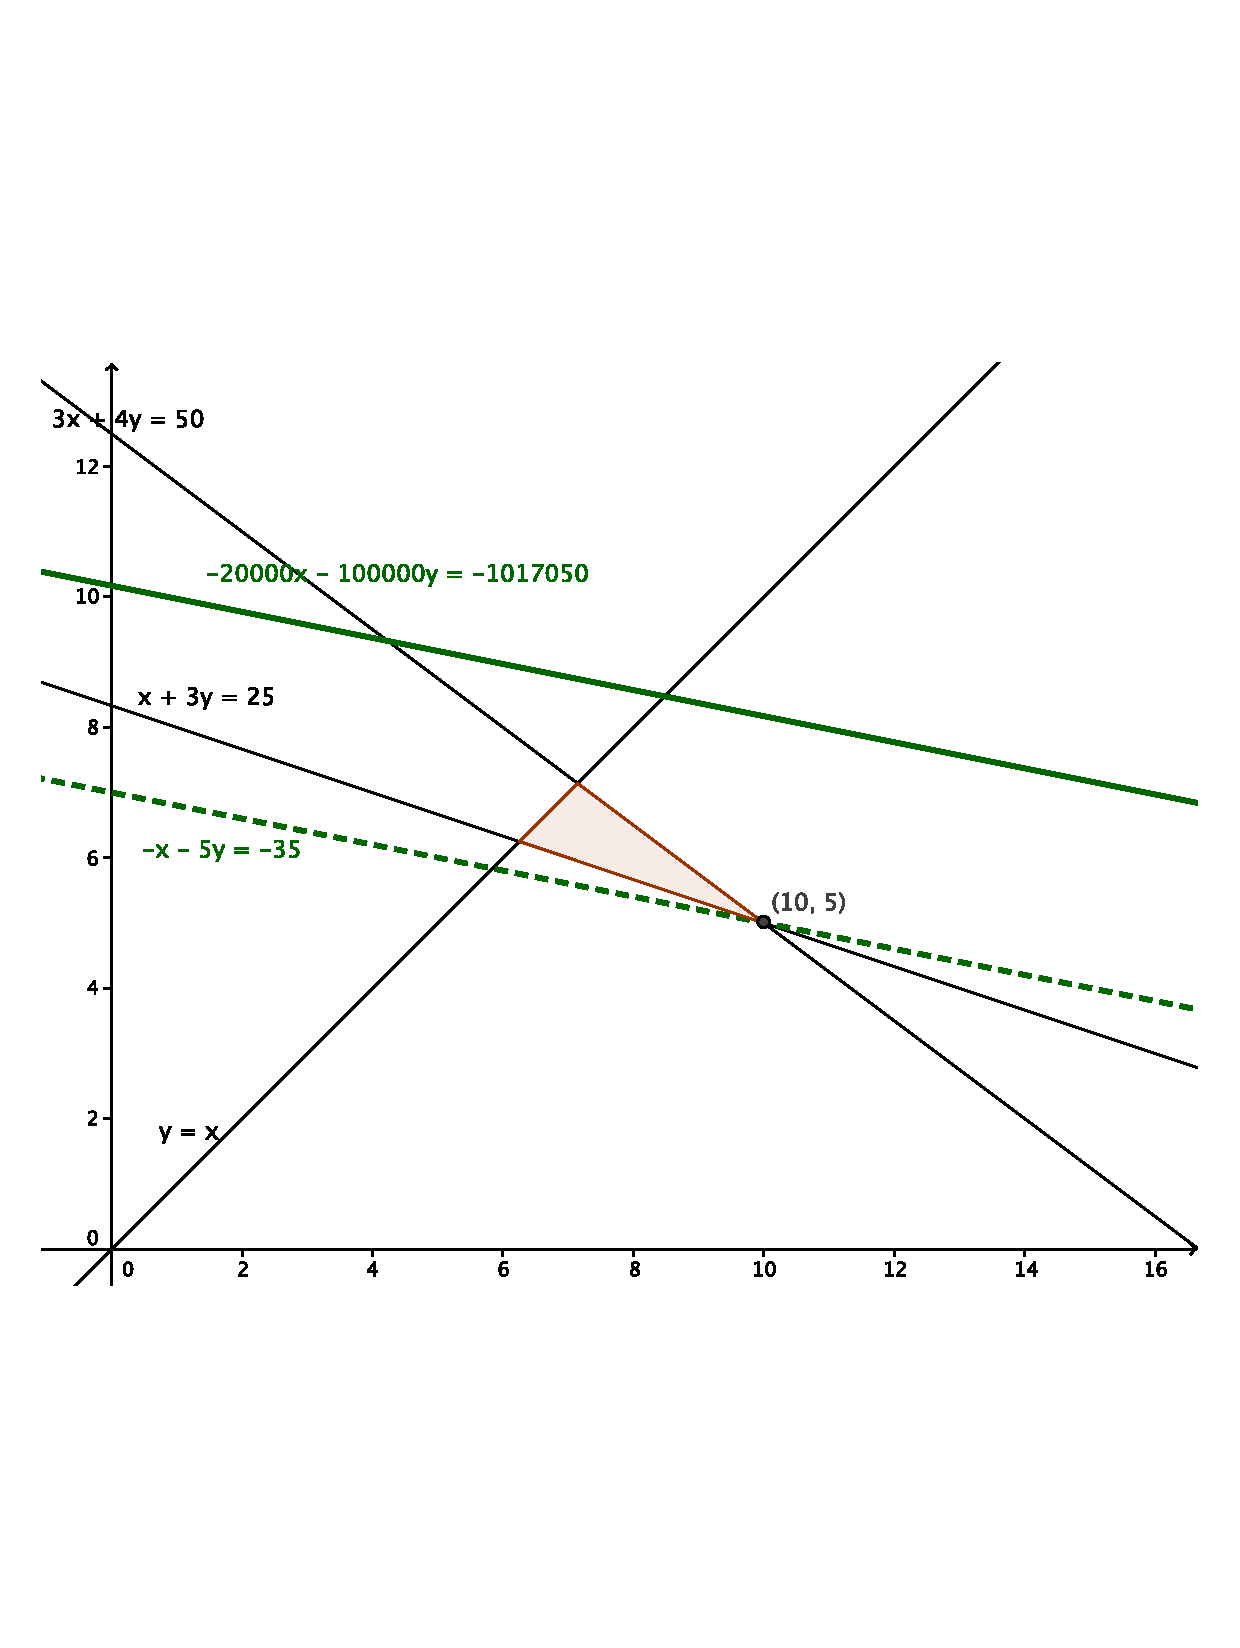
\includegraphics[width=0.8\textwidth]{oefeningen/FigurenLP/OefDepvhjaar.pdf}
\caption{Optimaal punt is 10 Fokkers en 5 Boeings}
\label{fig:deptjaar}
\end{figure}
\clearpage
\end{opl}
\end{oef}      

\begin{oef}
Artsen zonder Grenzen plannen een konvooi om de
noodlijdende bevolking van een vluchtelingenkamp in Afghanistan te 
bevoorraden met tenten en dekens, zodat de mensen de winter kunnen 
doorkomen. Per tent worden minstens drie dekens geleverd. Het totale laadvermogen van alle voertuigen samen is 
10 ton. Een tent weegt 2 kg en een deken 1 kg. Er zijn slechts 8000 dekens beschikbaar. Met een tent kan men 
5 vluchtelingen helpen, met een deken slechts \'{e}\'{e}n 
vluchteling. Hoeveel tenten en dekens moet men leveren om zoveel 
mogelijk mensen te helpen? 
\begin{opl}
Met 2000 tenten en 6000 dekens kunnen in totaal 16\,000 mensen geholpen worden (figuur~\ref{fig:AZG}).
\begin{figure}[hbtp]
  \centering
  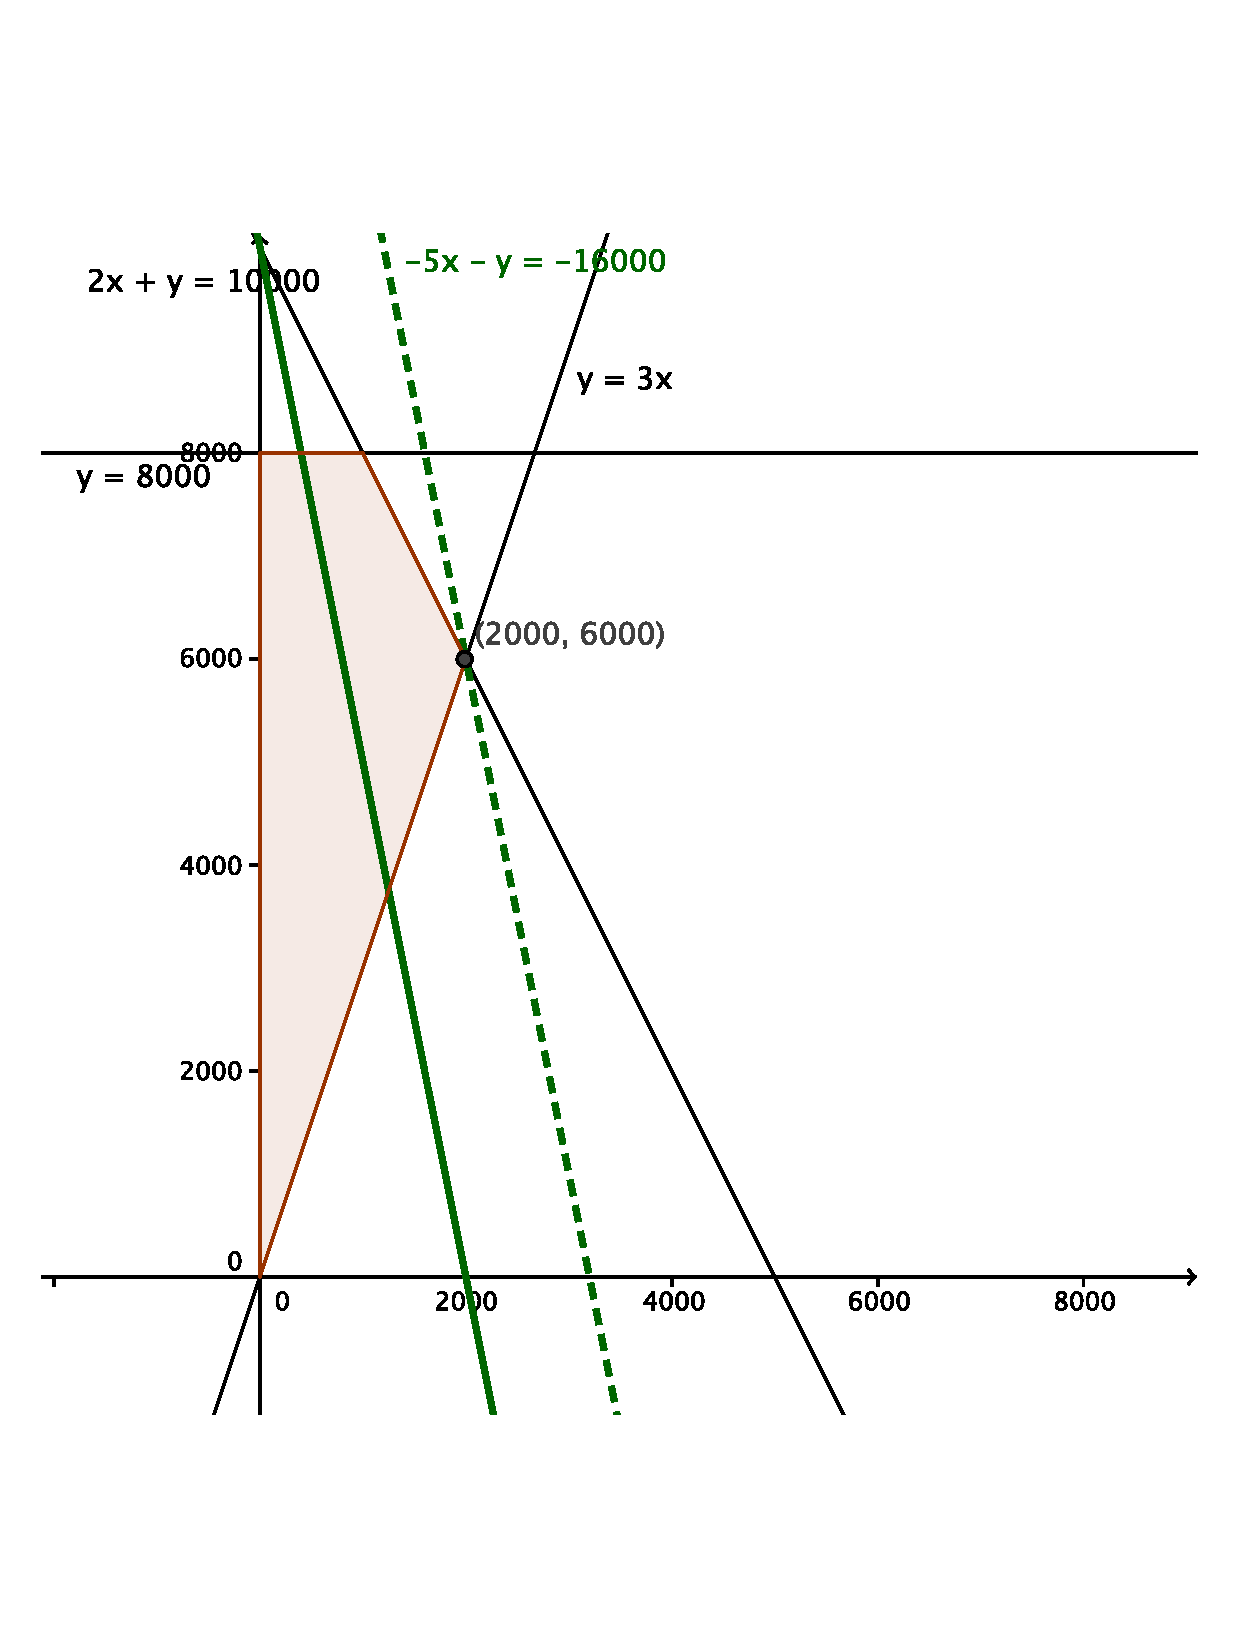
\includegraphics[width=0.7\textwidth]{oefeningen/FigurenLP/OefAZG.pdf}
  \caption{Optimaal punt is 2000 tenten en 6000 dekens}
  \label{fig:AZG}
\end{figure}
\end{opl}
\end{oef}
     
\begin{oef} \label{oef:toy-story}
In een speelgoedfabriek worden Woody
en Buzz Lightyear poppen gemaakt. 
\begin{figure}[ht]
  \centering
    
\includegraphics[scale=0.5]{oefeningen/FigurenLP/Buzz-Woody.jpg}
\end{figure}
Omwille van beperkingen van machines
kunnen er dagelijks in totaal maximaal 100 poppen gemaakt worden. De
directie van de fabriek heeft besloten om minstens 10 Buzz Lightyear
poppen en hoogstens 80 Woody poppen te maken per dag. 
De milieubijdrage
voor een Buzz Lightyear pop is 2 euro terwijl die maar de helft
bedraagt voor een Woody pop. De directie wil dagelijks niet meer dan 130
euro voorzien als milieubijdrage. Wegens de grotere populariteit van
Woody, worden er minstens evenveel Woody poppen gemaakt als Buzz
Lightyear poppen. Het bedrijf maakt een winst van 20 euro per Woody pop
en 10 euro per Buzz Lightyear pop.
\begin{enumerate}
  \item Bepaal de optimale dagelijkse productie van Woody en Buzz
        Lightyear poppen zodat het bedrijf een maximale winst heeft.
        (\textit{Je mag hierbij van uitgaan dat alle geproduceerde poppen ook
        effectief zullen worden verkocht en dus winst opleveren.}) Vermeld
        duidelijk en gedetailleerd welke stappen je hebt gevolgd om tot je
        oplossing te komen.
  \item Bereken de bijhorende maximale winst.
\end{enumerate}
\begin{opl}
Beperkingen
\[
  \begin{array}{r@{\;}c@{\;}l@{\hspace{2cm}}r@{\;}c@{\;}l}
    &&&                            \multicolumn{3}{c}{\mathbf{standaardvorm}} \\
    x & \geq & 0                   & x & \geq & 0 \\
    y & \geq & 0                   & y & \geq & 0 \\
    x + y & \leq & 100             & y & \leq & 100 - x \\
    y & \geq & 10                  & y & \geq & 10 \\
    x & \leq & 80                  & x & \leq & 80 \\
    x + 2y & \leq & 130            & y & \leq & 65 - 1/2x \\
    x & \geq & y                   & y & \leq & x \\
  \end{array}
\]
Doelfunctie (te maximaliseren)
\[
  W = 20x+10y \iff y = -2x + 1/10W
\]
Grafiek in \cref{fig:toy-story}. Optimale oplossing: 80 Woody poppen, 20 Byzz Lightyear poppen voor \euros{1800} opbrengst.
\begin{figure}[hbtp]
  \centering
  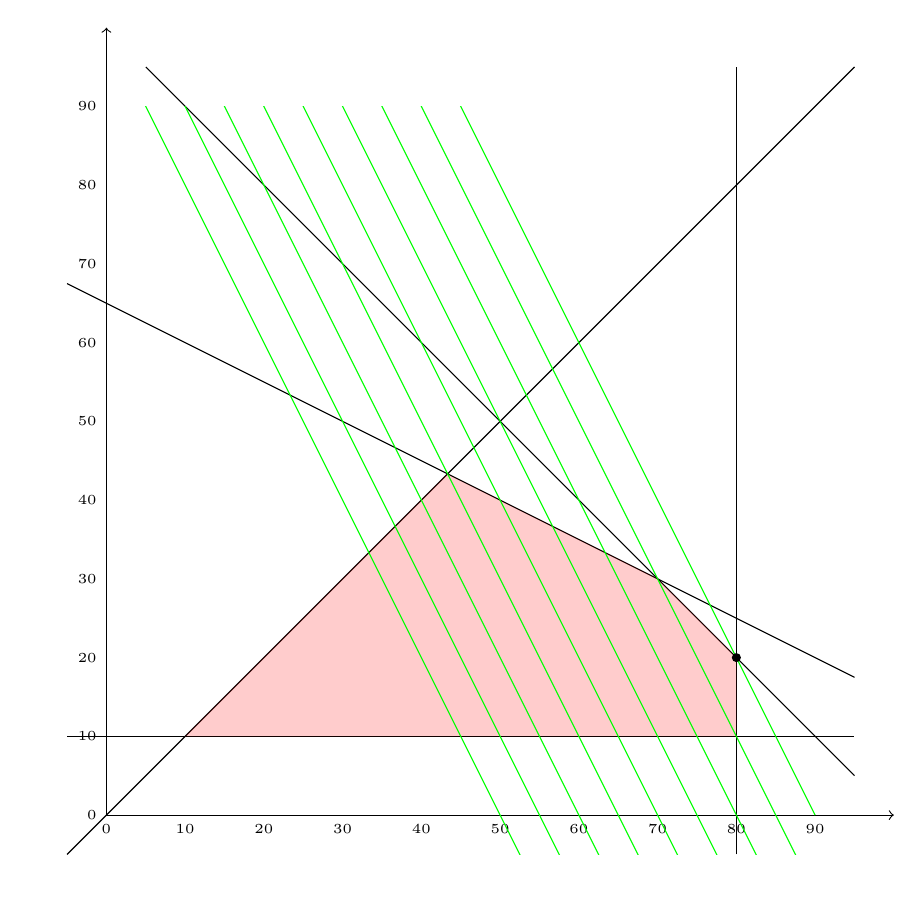
\begin{tikzpicture}
    \path[use as bounding box] (-1,-1) rectangle (10,10);
    \draw[->] (0,0) -- (10,0);
    \draw[->] (0,0) -- (0,10);
    \begin{scope}[scale=0.1]
      \foreach \c in {0,10,...,90} {
        \node[anchor=north] at (\c,0) {\tiny \c};
        \node[anchor=east] at (0,\c) {\tiny \c};
      }
      \draw[domain=5:95,smooth,variable=\x,black] plot ({\x},{100-\x});
      \draw[domain=-5:95,smooth,variable=\x,black] plot ({\x},{10});
      \draw[domain=-5:95,smooth,variable=\y,black] plot ({80},{\y});
      \draw[domain=-5:95,smooth,variable=\x,black] plot ({\x},{65-0.5*\x});
      \draw[domain=-5:95,smooth,variable=\x,black] plot ({\x},{\x});

      \fill[red,opacity=.2] (10,10) -- (80,10) -- (80,20) -- (70,30) -- (43.3,43.3) -- cycle;

      \begin{scope}
        \clip (-5,-5) rectangle (100,90);
        \foreach \W in {100,110,...,180} {
          \draw[domain=0:90,smooth,variable=\x,green!100!black!100] plot ({\x},{-2*\x+\W});
        }
      \end{scope}

      \draw[fill=black] (80,20) circle (.5cm);
    \end{scope}
  \end{tikzpicture}
  \caption{Visualisatie van \cref{oef:toy-story}}
  \label{fig:toy-story}
\end{figure}
\end{opl}
\end{oef}
  
\begin{oef}\label{oef:mais-rijst}
Een boer wil hoogstens 40 ha van zijn land bebouwen met
ma\"{i}s en aardappelen. Uit ervaring weet hij dat per ha ma\"is
$3$ dagen (hand)werk mag gerekend worden en per ha aardappelen 10 dagen.
Volgens zijn werkschema kan hij hoogstens 240 werkdagen besteden
aan het met de hand bewerken van ma\"is en aardappelen. De machines
bezit hij samen met andere boeren zodat hij slechts gedurende 47
extra dagen over de nodige machines kan beschikken. Voor de 
ma\"{i}s kan men per dag  \'e\'en ha bewerken met 
machines en voor 
de aardappelen bewerkt men per dag $\frac{2}{3}$ van een ha. 
Uiteindelijk  moet het aandeel van de ma\"{i}s minstens  \'e\'en
derde van de totale bewerkte oppervlakte zijn. De opbrengst
per ha voor ma\"is \euros{1000} is en die van aardappelen \euros{3000}.
Bepaal de verdeling van bewerkte oppervlakte ma\"is en
aardappelen die een maximale opbrengst levert. Bereken ook die
opbrengst. 
\begin{opl}
Beperkingen
\[
  \begin{array}{r@{\;}c@{\;}l@{\hspace{2cm}}r@{\;}c@{\;}l}
    &&& \multicolumn{3}{c}{\mathbf{standaardvorm}} \\
    x & \geq & 0 &            x & \geq & 0\\
    y & \geq & 0 &            y & \geq & 0 \\
    x + y & \leq & 40 &       y & \leq & 40 - x \\
    3x + 10y & \leq & 240 &   y & \leq & -3/10x+24\\
    x+3/2y & \leq & 47 &      y & \leq & -2/3x+94/3 \\
    x & \geq & 1/3(x+y) &     y & \leq & 2x \\
  \end{array}
\]
Doelfunctie (te maximaliseren)
\[
  W = 1000x+3000y \qquad \iff \qquad y = -1/3x + W/3000
\]
Grafiek in \cref{fig:mais-en-rijst}. Optimale oplossing: 20 ha ma\"is, 18 ha aardappelen voor \euros{74.000} opbrengst.
\begin{figure}[hbtp]
  \centering
  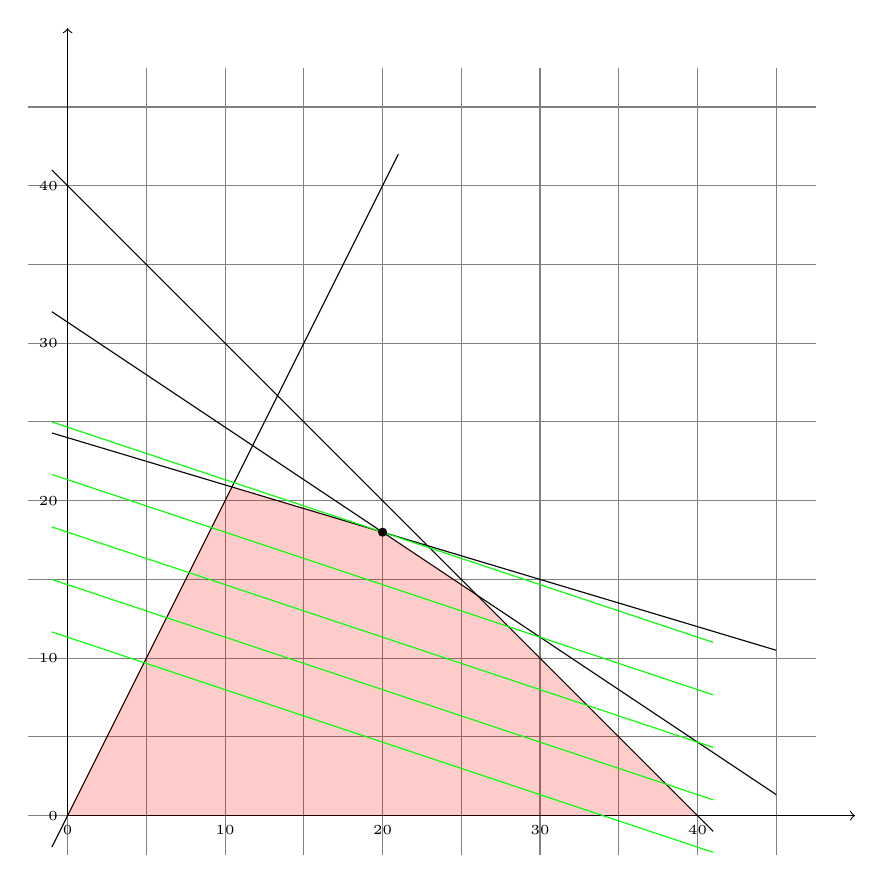
\begin{tikzpicture}
    \draw[gray,thin,step=1cm] (-.5,-.5) grid (9.5,9.5);
    \draw[->] (0,0) -- (10,0);
    \draw[->] (0,0) -- (0,10);
    \begin{scope}[scale=0.2]
      \foreach \c in {0,10,...,40} {
        \node[anchor=north] at (\c,0) {\tiny \c};
        \node[anchor=east] at (0,\c) {\tiny \c};
      }
      \draw[domain=-1:41,smooth,variable=\x,black] plot ({\x},{40-\x});
      \draw[domain=-1:45,smooth,variable=\x,black] plot ({\x},{-0.3*\x+24});
      \draw[domain=-1:45,smooth,variable=\x,black] plot ({\x},{-2/3*\x+94/3});
      \draw[domain=-1:21,smooth,variable=\x,black] plot ({\x},{2*\x});

      \fill[red,opacity=.2] (0,0) -- (10.4348,20.8696) -- (20,18) -- (26,14) -- (40,0) -- cycle;

      \foreach \W in {34,44,...,74} {
        \draw[domain=-1:41,smooth,variable=\x,green!100!black!100] plot ({\x},{-1/3*\x+\W/3});
      }

      \draw[fill=black] (20,18) circle (.25cm);
    \end{scope}
  \end{tikzpicture}
  \caption{Visualisatie van \cref{oef:mais-rijst}}
  \label{fig:mais-en-rijst}
\end{figure}
\end{opl}
\end{oef}
     
     
\begin{oef}
In een bedrijf produceert men tafels en stoelen. Voor de
productie van \'e\'en tafel is 3 maal zoveel hout nodig als
voor de productie van \'e\'en stoel. Er is in het bedrijf voldoende
hout aanwezig om per week 45 stoelen te maken. Een stoel vraagt echter
heel wat afwerking, zodat er voor het maken van \'{e}\'{e}n
stoel 2 maal zoveel personeel nodig is als voor een tafel. Het
bedrijf beschikt over net voldoende personeel om 20 stoelen af te
werken per week. De vraag naar tafels en stoelen samen, per week,
is 10 stuks, zodat het bedrijf per week minstens 10 meubelstukken zal produceren. De winst per tafel is \euros{125} en die per stoel is
\euros{75}. Hoeveel tafels en stoelen moet men produceren om de
winst zo groot mogelijk te maken? Hoeveel bedraagt de winst?
\begin{opl}
10 tafels en 15 stoelen (figuur~\ref{fig:tafelstoelen}) leveren de grootste winst, nl \euros{2375}.
\begin{figure}[hbtp]
\centering
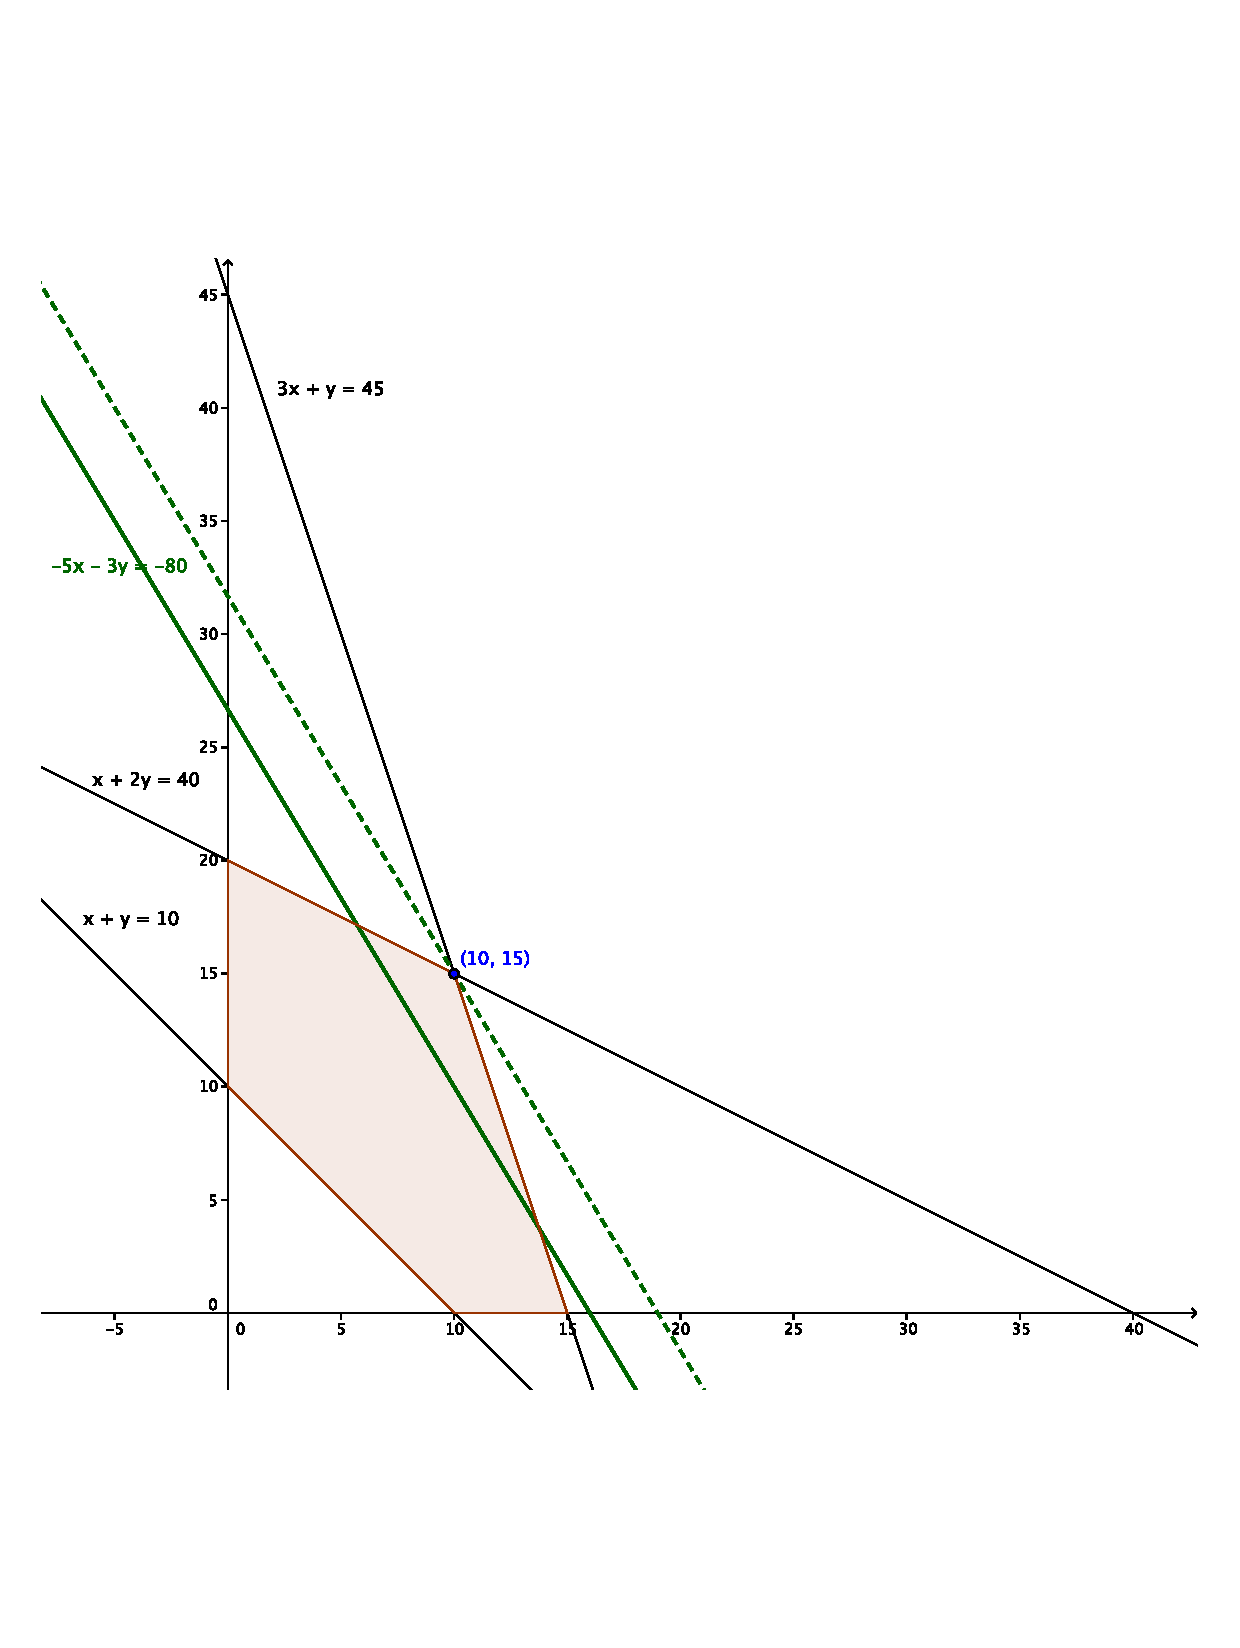
\includegraphics[width=0.8\textwidth]{oefeningen/FigurenLP/Oef7.pdf}
\caption{10 tafels en 15 stoelen leveren de grootste winst}
\label{fig:tafelstoelen}
\end{figure}
\clearpage
        \end{opl}
\end{oef}

     
\begin{oef}
Een bedrijf produceert 2 types containers.
Voor de productie van 
\'{e}\'{e}n container van type A is driemaal zoveel personeel 
nodig als voor \'{e}\'{e}n container van type B. Het bedrijf 
beschikt over voldoende personeel om 120 containers van type B te 
maken per dag. Voorts vereist \'{e}\'{e}n container van type B 
tweemaal zoveel staal als \'{e}\'{e}n container van type A. Er is 
in het bedrijf voldoende staal aanwezig om per dag 60 containers 
van type A te maken. De winst per container van type A is \euros {2500} 
en die per container van type B is \euros{1000}. Er is elke dag 
vraag naar \emph{minstens} 15 containers van beide types samen. Het 
aandeel van containers van type A is minstens \'{e}\'{e}n  vierde 
van de dagelijkse productie van beide types containers \emph{samen}. 
\emph{Hoeveel} containers van type A en hoeveel van type B moet 
het bedrijf produceren om de winst zo groot mogelijk te maken?
\begin{opl}
De maximale winst (\euros{102\,000}) wordt bereikt bij de productie van 36 containers van type A en 12 containers van type B (figuur~\ref{fig:containersAB}).
\begin{figure}[hbtp]
\centering
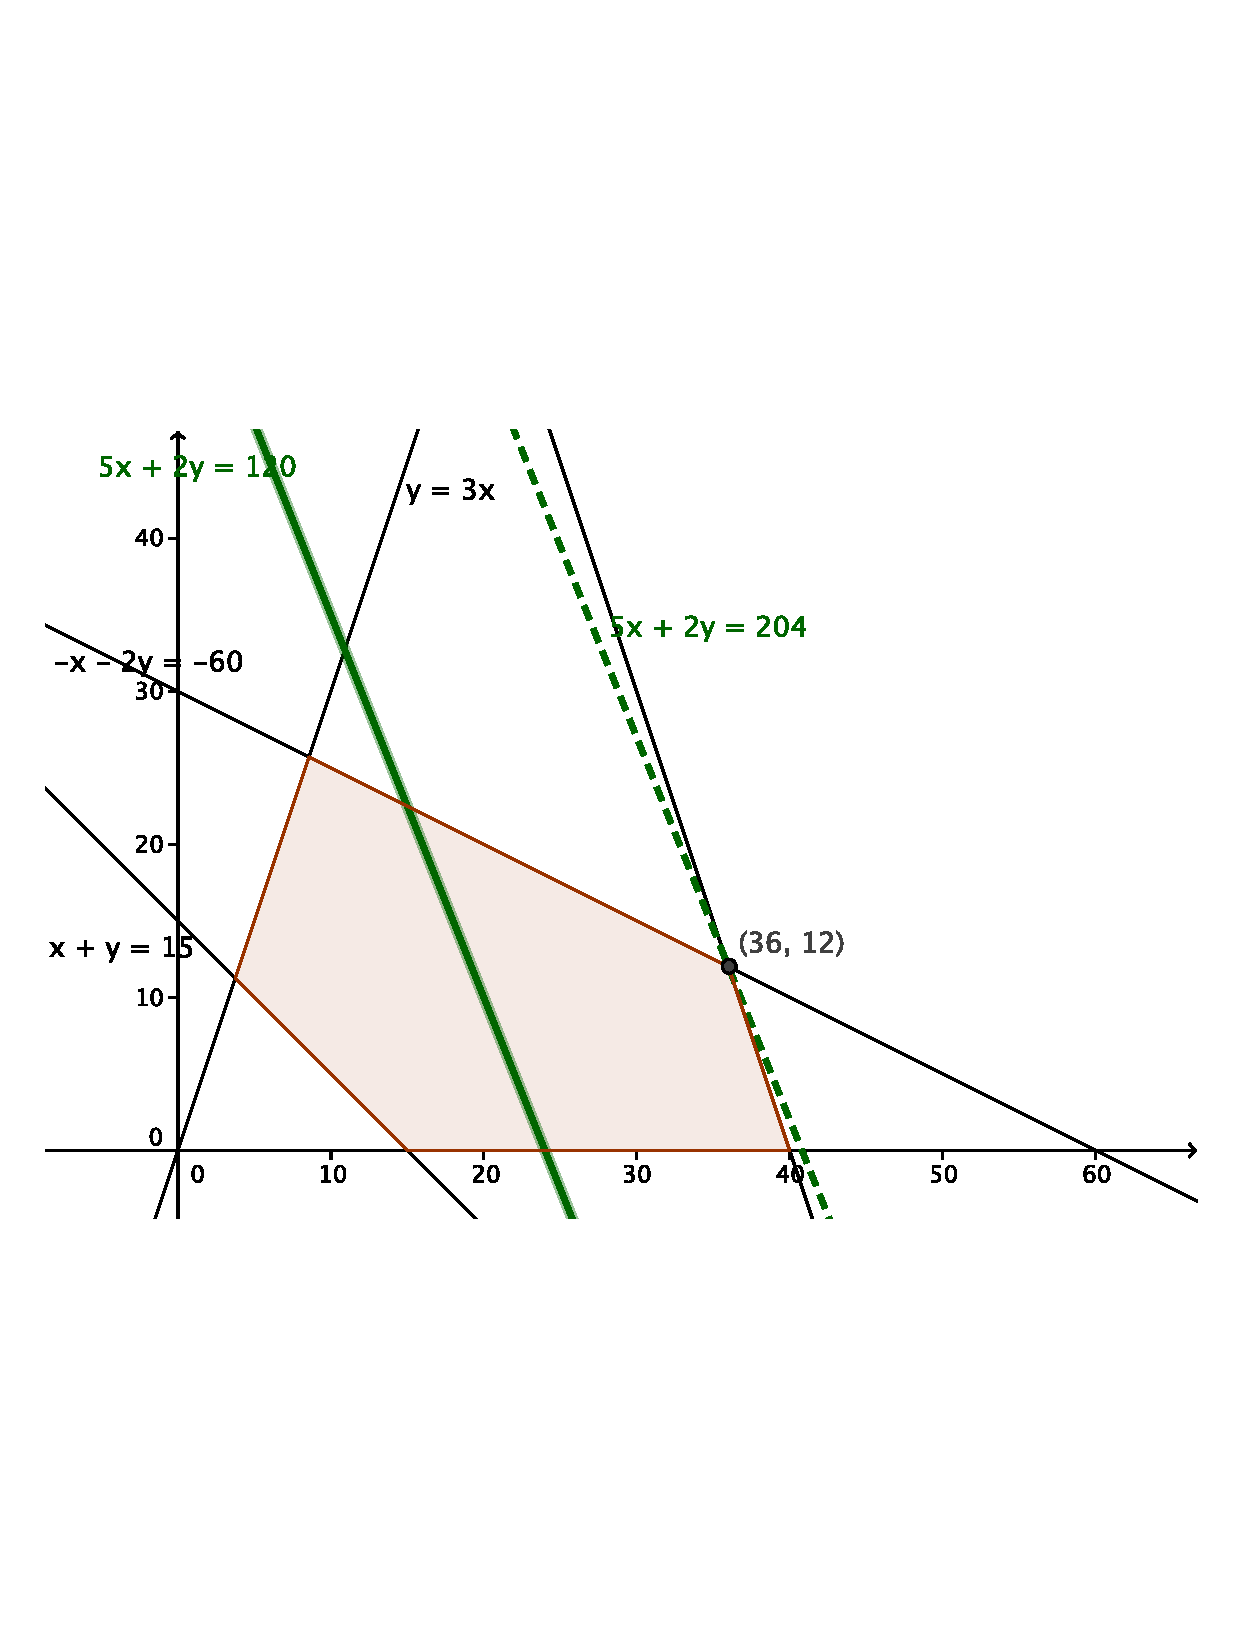
\includegraphics[width=0.8\textwidth]{oefeningen/FigurenLP/OefcontainersAB.pdf}
\caption{De grootste winst is bij 36 containers A en 12 containers B}
\label{fig:containersAB}
\end{figure}
    \end{opl}
\end{oef}

\begin{oef}
Een fabriek produceert metalen platen en buizen.
Het aantal machines voor deze productie laat toe om maximaal 35
ton platen \emph{of} 70 ton buizen per maand te maken. Hiervoor zijn 80
arbeiders beschikaar. E\'en man kan per maand 1 ton platen \emph{of} 500
kg buizen verwerken. De buizen vereisen een nabehandeling in een
andere afdeling waar slechts 35 ton per maand kan afgewerkt
worden.   De opbrengst voor de fabriek op \'e\'en ton platen en
\'e\'en ton buizen is respectievelijk \euros{2500} en
\euros{2000}. Bepaal  de optimale
productie waardoor de fabriek een maximale opbrengst bekomt. 
\begin{opl}
Een maandproductie van 20 ton platen en 30 ton buizen (figuur~\ref{fig:platenbuizen}) levert de maximale winst van \euros{110\,000}.
                 \begin{figure}[hbtp]
\centering
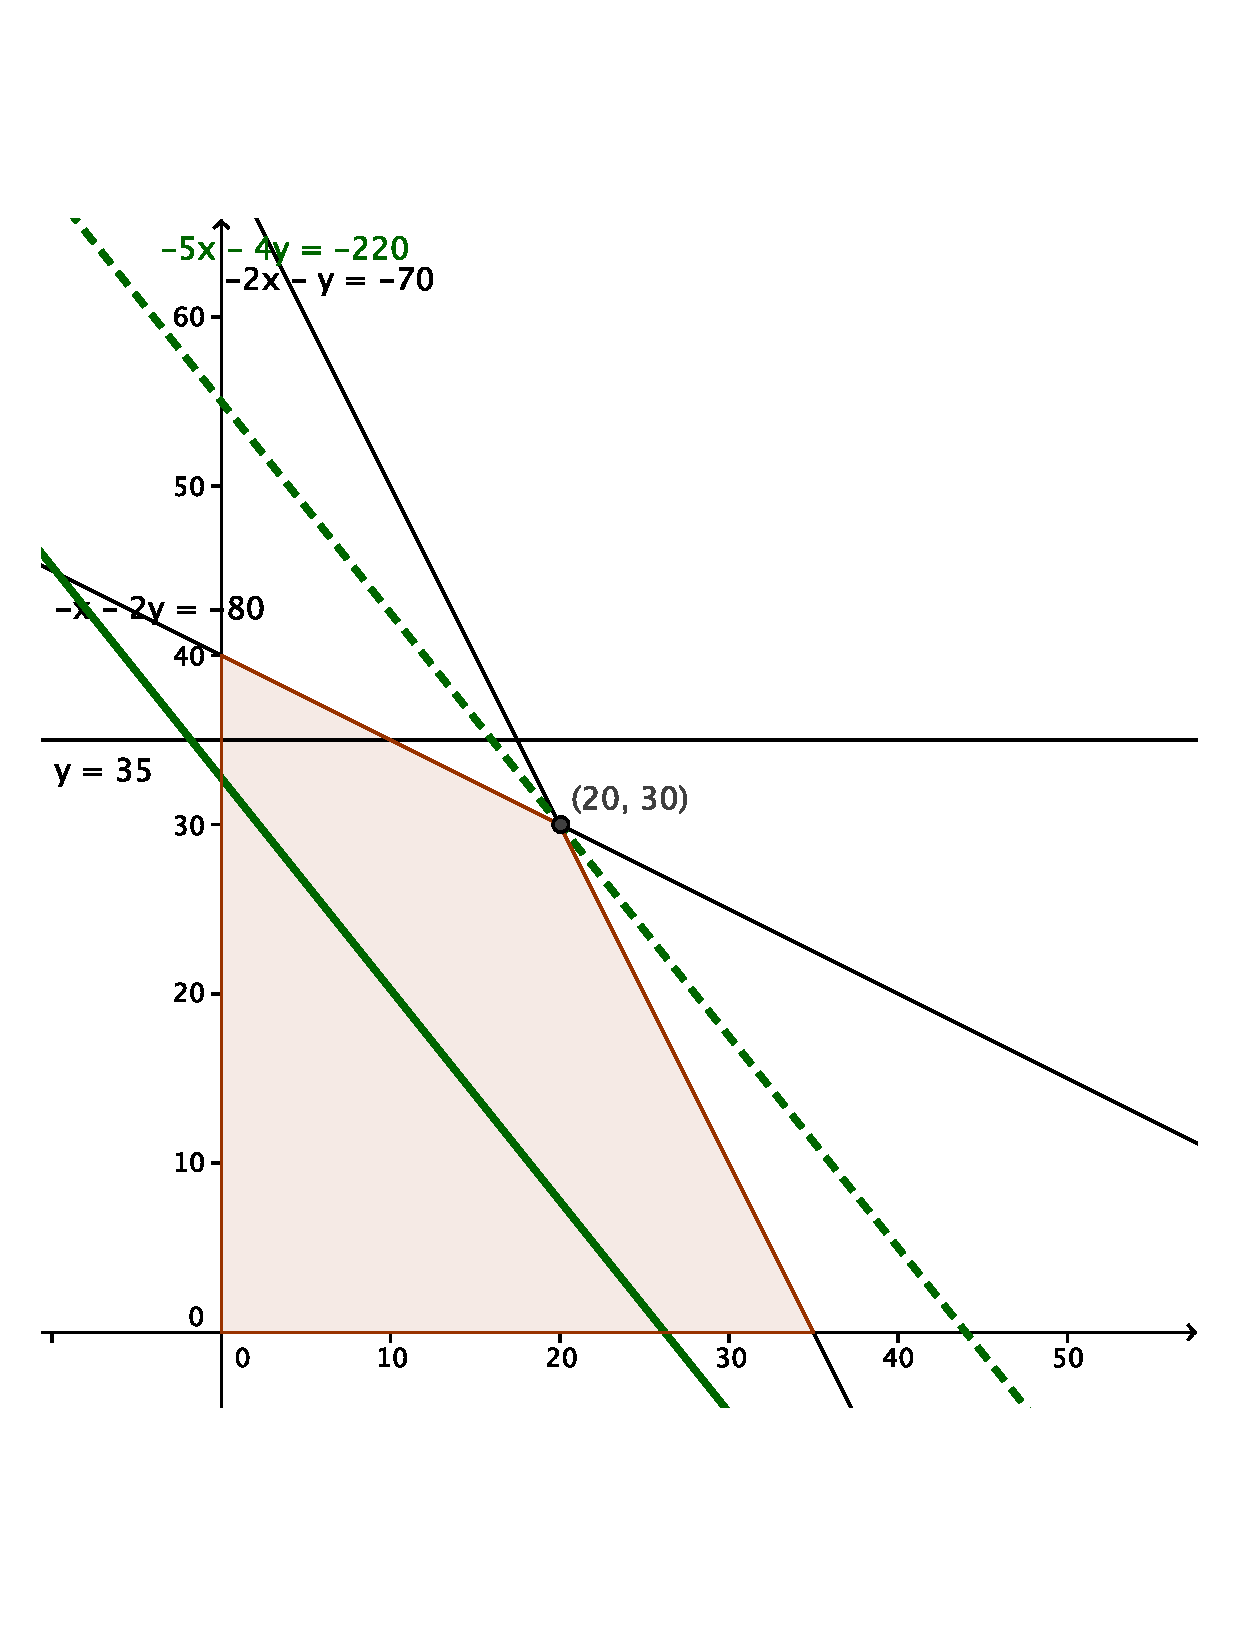
\includegraphics[width=0.8\textwidth]{oefeningen/FigurenLP/OefPlatenBuizen.pdf}
\caption{Maximale winst bij 20 ton platen en 30 ton buizen}
\label{fig:platenbuizen}
\end{figure}
\clearpage
     \end{opl}
\end{oef}
     


\begin{oef}
Een bioscoopzaal draait voorlopig alleen 
    `The lord of de Rings (LR) en `Harry Potter en de steen der wijzen' (HP). Bij 
     voorstellingen van LR laat men maximaal 100 volwassenen en 50 
     kinderen toe (inkomprijs \euros{8} resp.\ \euros{6}). Bij HP is dat 
     40 volwassenen en 160 kinderen (inkomprijs \euros{7} resp.\ 
     \euros{4}).  De onkosten 
     (personeel, rechten, apparatuur\ldots) voor 
     een voorstelling van LR bedragen \euros{200} voor HP \euros{120}.  De 
     totale winst van alle voorstellingen samen moeten minstens 
     \euros{21600} bedragen. Het poetswerk na een vertoning van LR duurt 
     10 minuten en bij HP 20 minuten. Het poetspersoneel mag in totaal  
     maximum 7.5 uren werken. De filmdistributeur bepaalt dat het aantal 
     vertoningen van LR  maximum 30 bedraagt en minstens 
     evenveel als het aantal vertoningen van HP. We veronderstellen 
          dat alle vertoningen vol geboekt zijn.
     Hoeveel voorstellingen van elke film moet men geven opdat het aantal 
     kinderen dat naar de film kan zo groot mogelijk is? 
     \begin{opl}
     15 voorstellingen van elke film
     \end{opl}
\end{oef}
     

\begin{oef}
De directie van een pretpark buigt zich over de uitbreiding van het
parkeerterrein met een aanpalend stuk grond. Op de parking kunnen zowel auto's als autobussen parkeren. Voor de autobussen worden geen speciale plaatsen voorzien: zij nemen gewoon 3 autoparkeerplaatsen in.  Er is ruimte voor 75
personenauto's.  Er worden maximaal 10 bussen toegelaten op de parking. 
Per bus moeten minstens 3 auto's toegelaten worden en mogen er maximaal 8 auto's parkeren.  Per dag levert een auto \euros{4}
parkeergeld op, een autobus \euros{15}. Hoeveel auto's en bussen moeten er op de parking parkeren opdat de opbrengst per dag maximaal zou zijn? 
\begin{opl}
Als de parking dagelijks 45 auto's en 10 bussen ontvangt (figuur~\ref{fig:autobussen}), is de opbrengst maximaal (\euros{330}).
                 \begin{figure}[hbtp]
\centering
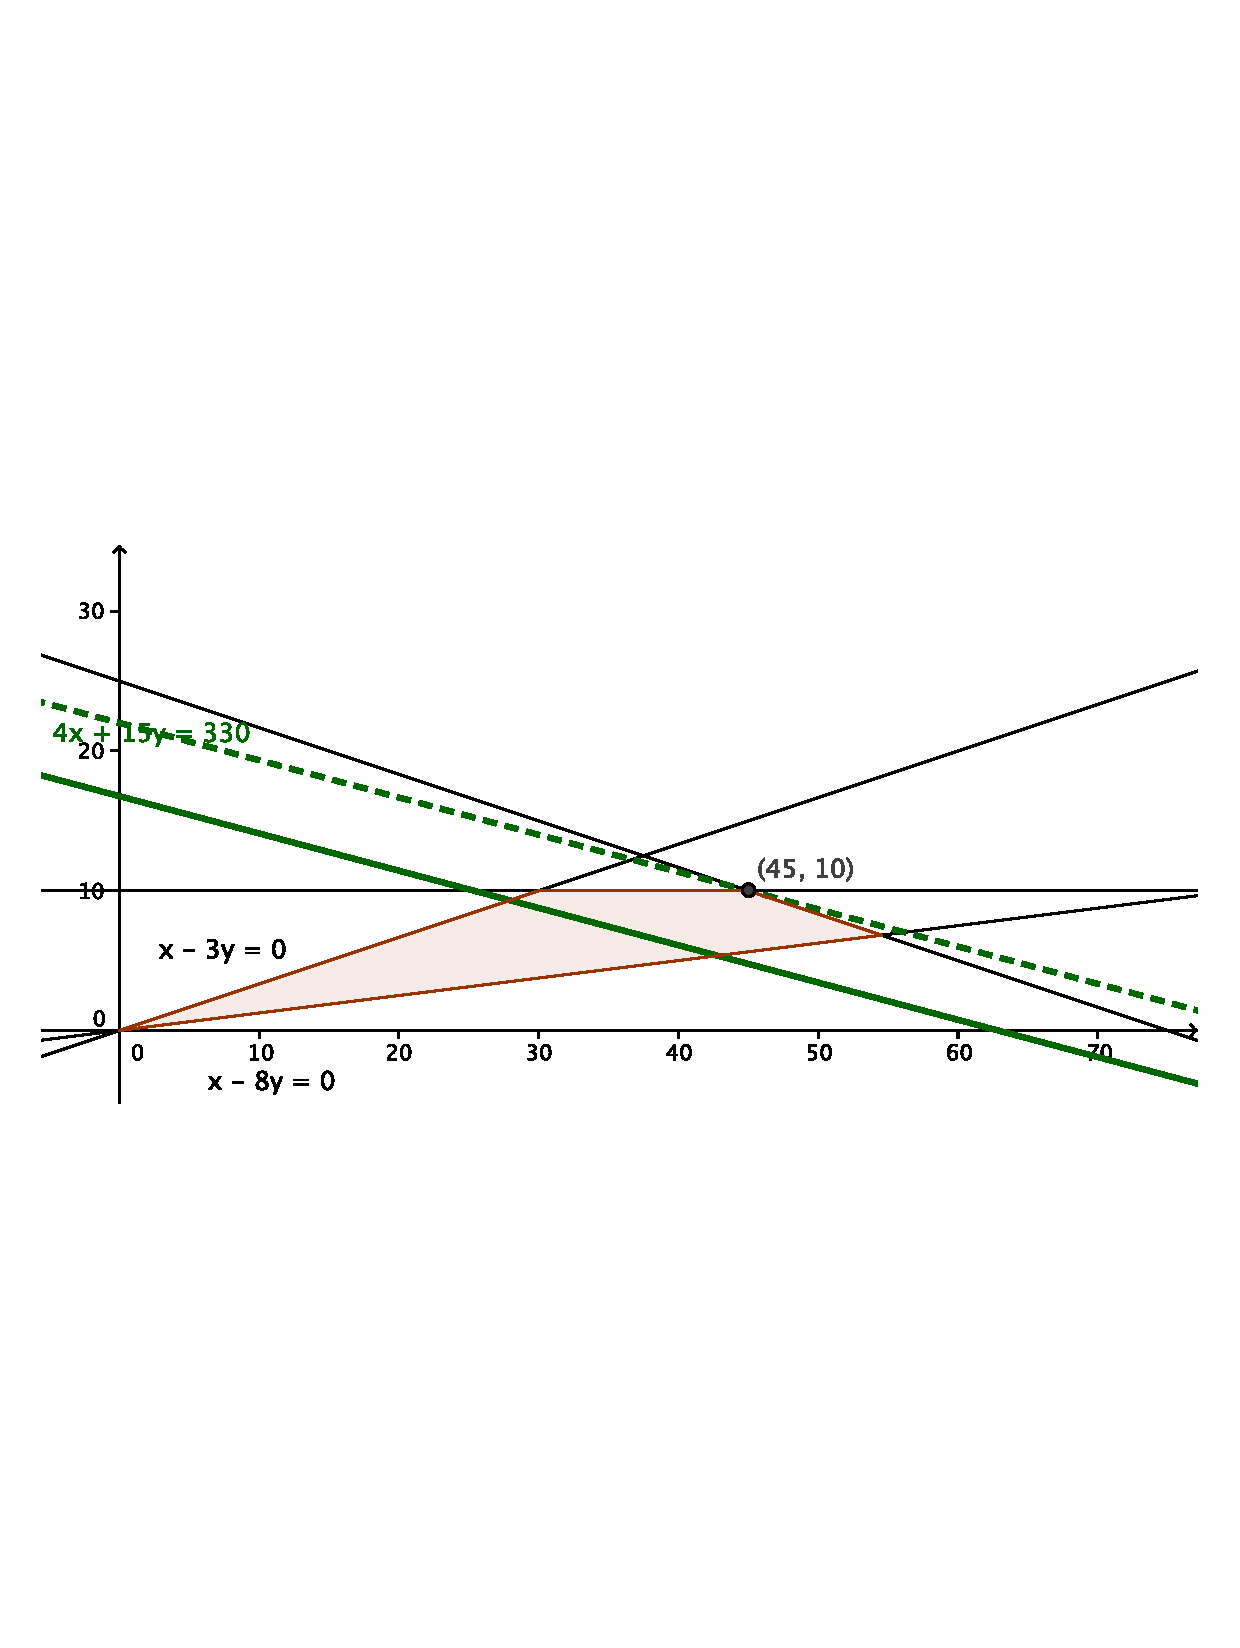
\includegraphics[width=0.8\textwidth]{oefeningen/FigurenLP/Oefautosbussen.pdf}
\caption{Maximale parkingopbrengst bij 45 auto's en 10 bussen}
\label{fig:autobussen}
\end{figure}
\end{opl}
\end{oef}

\begin{oef}
Voor een sponsoractie op school vult Anne potjes met vanille- en chocoladepudding. 
Haar moeder heeft 40 potjes die ze kan vullen 
(maar ze moeten niet allemaal gevuld worden).
Anne heeft de juf beloofd om minstens 25 potjes mee te brengen.
Ze denkt dat meer mensen vanillepudding lusten dan chocoladepudding,
dus vult ze minstens evenveel potjes met vanille als chocolade.
Vanillepudding afwerken vraagt dubbel zoveel tijd als chocoladepudding
afwerken. Anne heeft tijd om 70 potjes chocoladepudding af te werken.
Ze verkoopt de potjes vanillepudding aan \euros{1} het stuk en de 
chocoladepudding aan \euros{0,80}.
Hoeveel potjes moet Anne van elk verkopen om zoveel mogelijk
opbrengst te bekomen? 
\begin{opl}
Als Anne 30 potjes vanille- en 10 potjes chocoladepudding maakt en verkoopt (figuur~\ref{fig:pudding}) heeft ze een maximale opbrengst van \euros{38}.
\begin{figure}[hbtp]
\centering
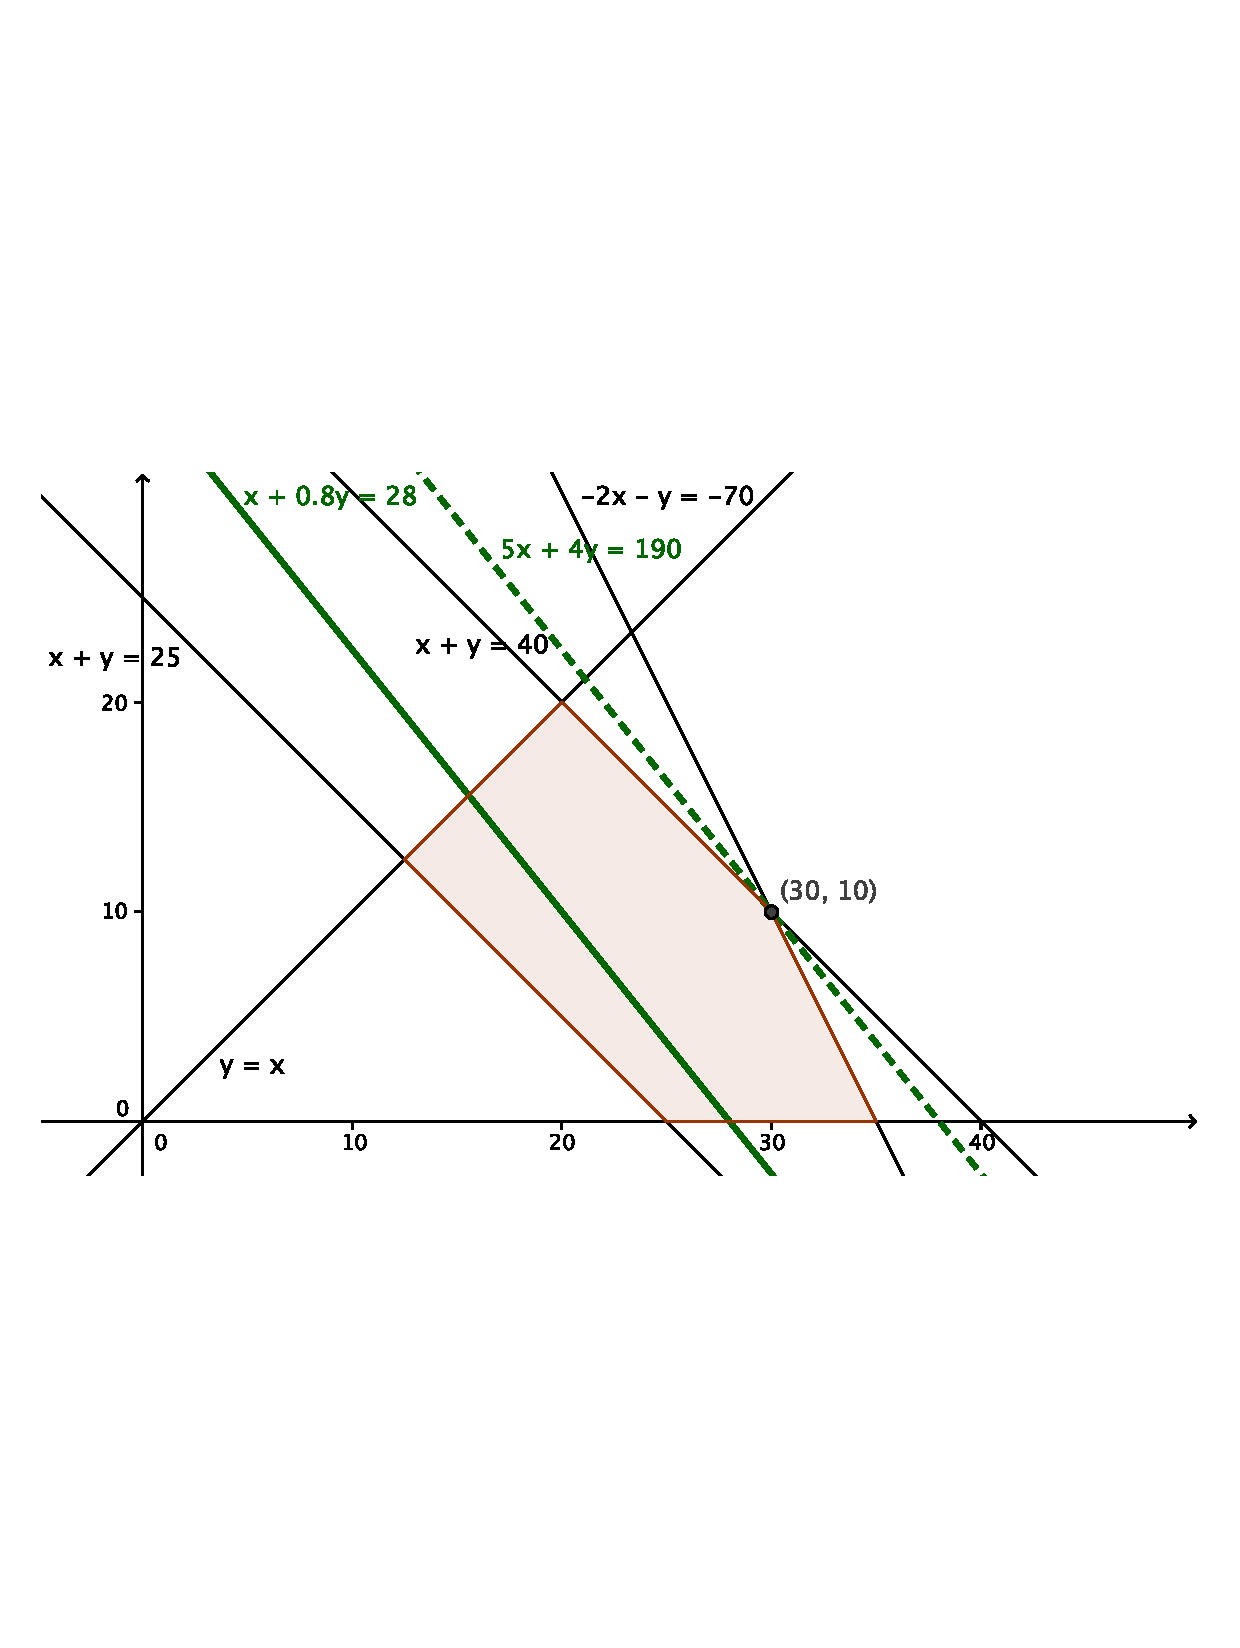
\includegraphics[width=0.8\textwidth]{oefeningen/FigurenLP/Oefpudding.pdf}
\caption{Maximale winst bij 30 potjes vanille- en 10 chocoladepudding}
\label{fig:pudding}
\end{figure}
\end{opl}
\end{oef}

\begin{oef}
Een houthakker kapt in het bos vogelkers en eik. 
De houthakker mag niet zoveel kappen als hij wil. De bosgroep hanteert
daarvoor een puntensysteem. Per ha mag er maar voor maximaal 21 punten
gehakt worden. Een vogelkers is 1 punt waard; een eik 3 punten.
Het bos is 5 ha groot.
Een eik is makkelijker te kappen dan een vogelkers. Als de houthakker per dag maar 
\'e\'en soort zou kappen, zou hij op \'e\'en dag 4 vogelkersen of 6 eiken kappen. 
Hij kan maximaal 10 dagen gaan werken in het bos.
Per eik mag de houthakker hoogstens 3 vogelkersen vellen.
Het aantal vogelkers moet minstens \'e\'en derde van het totaal aantal bomen
tellen.
Een eik geeft 10 keer zoveel winst als een vogelkers. Hoeveel bomen van elk soort
moet de houthakker kappen om zo veel mogelijk winst te bekomen? 
\begin{opl}
15 vogelkers, 30 eiken
\end{opl}
\end{oef}

\begin{oef}    
Een bouwbedrijf specialiseerde zich in het verbouwen van oude panden tot stijlvolle lofts en in de bouw van casco 1-slaapkamer appartementen. Het bedrijf heeft jaarlijks een budget van \SI{20000000}{\euro}. Om dit bedrag te kunnen lenen bij de bank moeten ze garanderen om minstens 10 appartementen en 50 lofts te realiseren. De bouw van een loft kost \SI{200000}{\euro}, een appartement is een stuk goedkoper, dit kost het bedrijf slechts \SI{100000}{\euro}. Het bouwbedrijf werkt nauw samen met een grote algemene aannemer. Deze aannemer kan maximaal personeel leveren voor de bouw van 60 lofts of 135 appartementen. De lofts kunnen anno 2013 verkocht worden aan \SI{300000}{\euro}. Voor een appartementje kan het bedrijf rekenen op een verkoopprijs van \SI{160000}{\euro}. Hoeveel lofts en appartementen moet het bedrijf realiseren en verkopen om zijn winst te maximaliseren?
\begin{opl}
50 lofts en 22 appartementen (eigenlijk 22,5 appartementen, maar je kan geen half appartement bouwen)
\begin{figure}[htb]
\centering
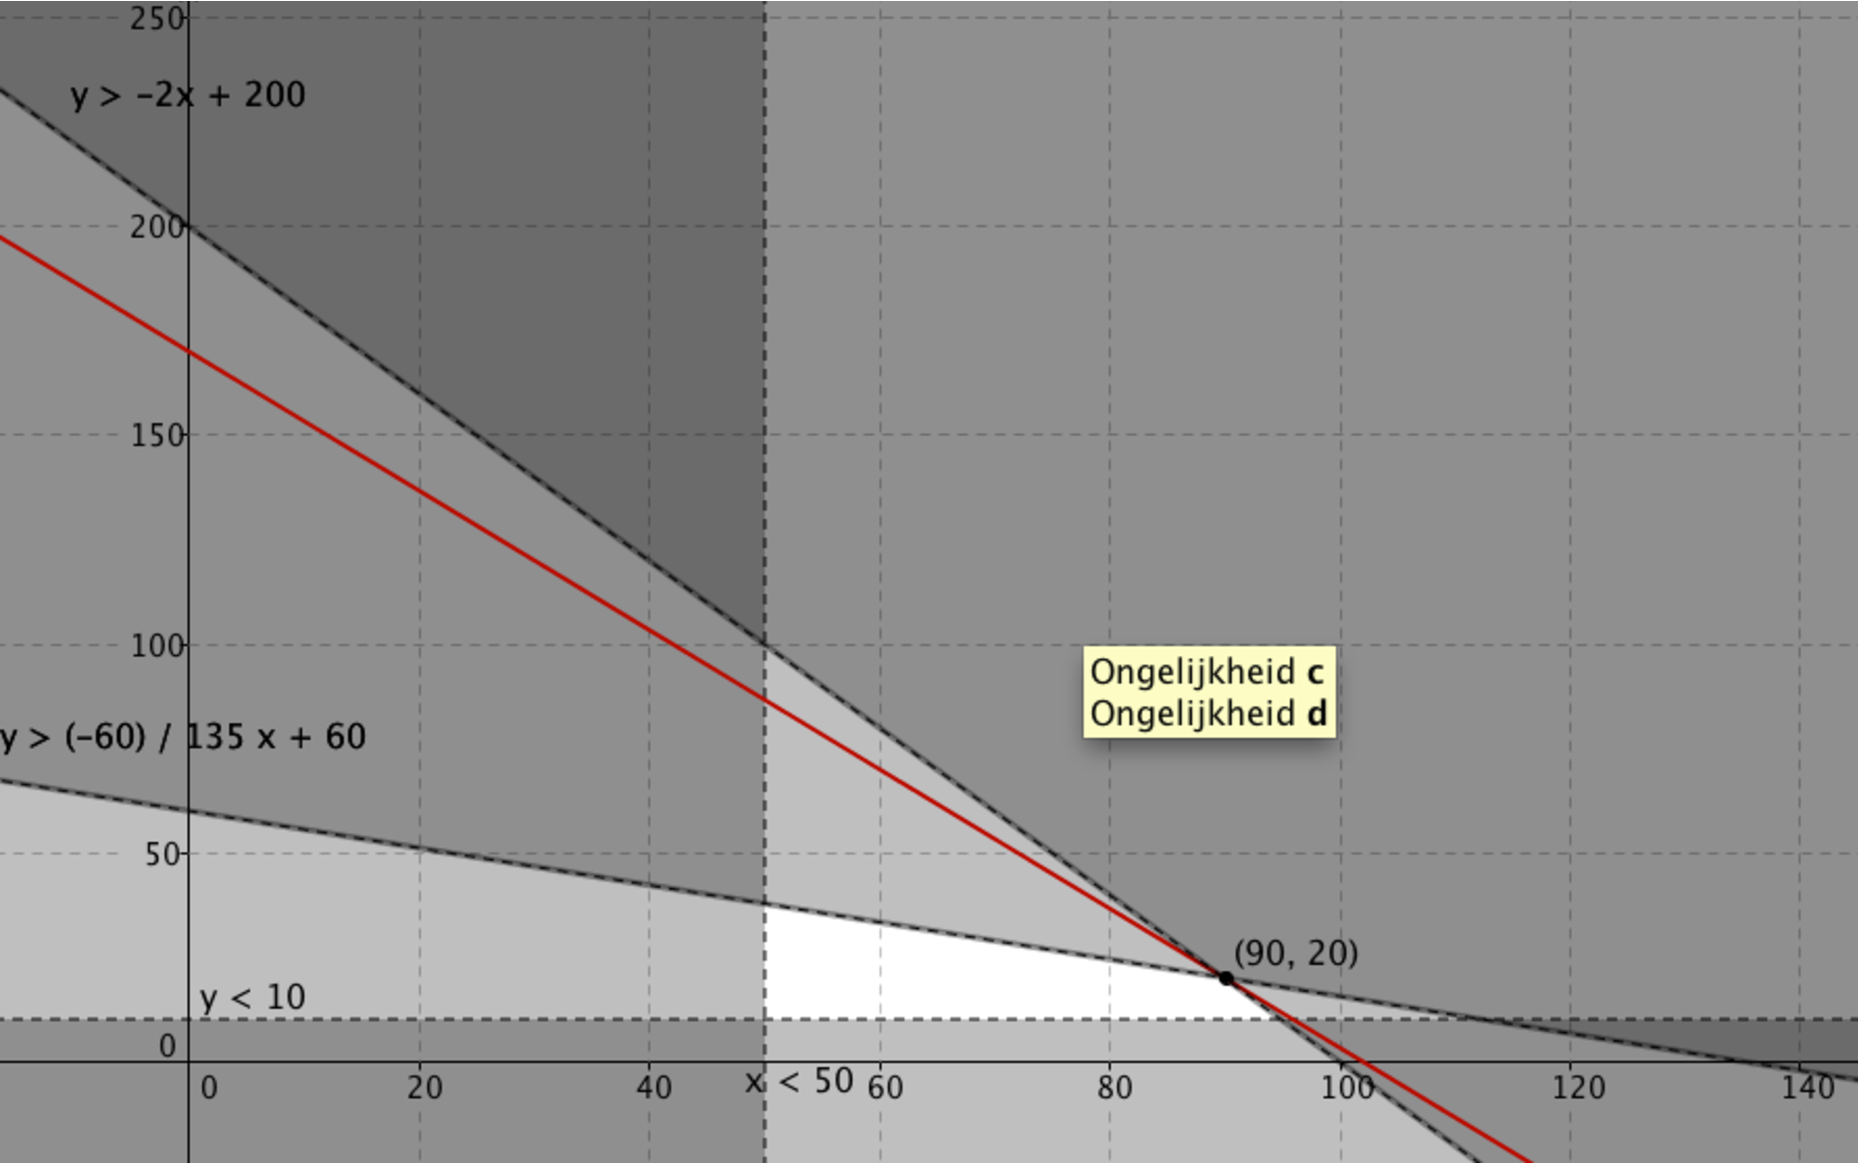
\includegraphics[width=0.8\textwidth]{oefeningen/FigurenLP/lofts}
\end{figure}
\end{opl}
\end{oef}




%%% Local Variables: 
%%% mode: latex
%%% TeX-master: "../cursusTW1"
%%% End: 
